\documentclass[a4j, titlepage]{jsarticle}
\usepackage[dvipdfmx]{graphicx}
\usepackage{amsmath,ascmac,amsthm, amssymb}
\usepackage{amsfonts,latexsym,mathtools}
\usepackage{bm}
\usepackage{algorithm,algorithmic}
\usepackage{listings}
\usepackage{empheq}
\lstset{
    language={C},
    basicstyle={\small\ttfamily},
    identifierstyle={\small},
    commentstyle={\small\itshape},
    keywordstyle={\small\bfseries},
    ndkeywordstyle={\small},
    stringstyle={\small\ttfamily},
    frame={tb},
    breaklines=true,
    columns=[l]{fullflexible},
    numbers=left,
    xrightmargin=0zw,
    xleftmargin=3zw,
    numberstyle={\scriptsize},
    stepnumber=1,
    numbersep=1zw,
    lineskip=-0.5ex
}
\renewcommand{\lstlistingname}{コード}
\renewcommand{\lstlistlistingname}{コード目次}

\numberwithin{equation}{section}
%\setcounter{tocdepth}{3}

\begin{document}
\begin{titlepage}
    \begin{center}
        {\Large 令和四年度後期 数理工学実験 課題レポート}

        \vspace*{180truept}

        {\Huge 熱方程式の差分法}

        \vspace{160truept}

        {\Large 情報学科2回生 平田蓮}

        \vspace{10truept}

        {\large 学生番号: 1029342830}

        \vspace{60truept}

        {\large 実験日: 10月25, 31日, 11月1, 7日}

        \vspace{10truept}

        {\large 実験場所: 京都大学工学部総合校舎数理計算機室}

        \vspace{60truept}

        {\large 11月14日 提出}
    \end{center}
\end{titlepage}

\tableofcontents
\clearpage

\section{目的}
    本実験では、熱方程式(拡散方程式)の差分法について学ぶ。

\section{原理}
    本節では、\ref{sec:ex}で行う課題で用いるアルゴリズムについて述べる。

    \subsection{拡散方程式}
        微粒子などが空間上で自発的に広がる現象を拡散といい、
        拡散方程式はその振る舞いを記す。
        ここでは1次元空間上の拡散を考える。
        微粒子の濃度を$C(x, t)$,
        流れを$J(x, t)$とする。
        微粒子の保存を考えると、
        \begin{equation}
            \frac{\partial}{\partial t}C(x, t) = -\frac{\partial}{\partial x}J(x, t) \label{equ:conservation}
        \end{equation}
        を得る。
        また、$J$は濃度勾配に比例すると考えると、
        比例定数$D$を用いて、
        \begin{equation}
            J(x, t) = -D\frac{\partial}{\partial x}C(x, t) \label{equ:slope}
        \end{equation}
        と書ける。これらを合わせて、拡散方程式
        \begin{equation*}
            \frac{\partial}{\partial t}C(x, t) = D\frac{\partial^2}{\partial x^2}C(x, t)
        \end{equation*}
        を得る。

        $D=1$として、方程式
        \begin{equation}
            \frac{\partial}{\partial t}u(x, t) = \frac{\partial^2}{\partial x^2}u(x, t) \label{equ:diffusion}
        \end{equation}
        を初期条件$u(x, 0) = u_0(x)$、範囲$x\in[0, L]$のもとで考える。
        これを解くには、初期条件の他に、$x=0,L$での境界条件が必要である。
        本実験では、主に以下の境界条件を用いる。

        \paragraph{Dirichlet境界条件}
            境界上の$u$の値を与える。
            \begin{eqnarray*}
                u(0, t) &=& u_L \\
                u(L, t) &=& u_R
            \end{eqnarray*}

        \paragraph{Neumann境界条件}
            境界上の$u$の傾きを与える。
            \begin{eqnarray*}
                \frac{\partial u}{\partial x}(0, t) &=& J_L \\
                \frac{\partial u}{\partial x}(L, t) &=& J_R \\
            \end{eqnarray*}

    \subsection{数値解法}
        時間と空間を離散化して式(\ref{equ:diffusion})を解くことを考える。
        時間と空間の刻み幅をそれぞれ$\Delta t, \Delta x$、
        空間の刻み数を$N$とする。($\therefore L = N\Delta x$)
        離散化された時空間上での$u$の平均値を、
        \begin{equation*}
            u_j^n \coloneqq \frac{1}{\Delta x}\int_{(j - 1)\Delta x}^{j\Delta x}u(x, n\Delta t)\mathrm{d}x \ (1 \leq j \leq N, 0 \leq n)
        \end{equation*}
        とする。$u_0^n, u_{N + 1}^n$を用いて境界条件を表す。

        \paragraph{Dirichlet境界条件}
            \begin{eqnarray*}
                u_0^n &=& u_L \\
                u_{N + 1}^n &=& u_R
            \end{eqnarray*}

        \paragraph{Neumann境界条件}
            \begin{eqnarray*}
                u_1^n - u_0^n = J_L\Delta x &\rightarrow& u_0^n = u_1^n - J_L\Delta x \\
                u_{N + 1}^n - u_N^n = J_R\Delta x &\rightarrow& u_{N + 1}^n = u_N^n + J_R\Delta x
            \end{eqnarray*}

        \subsubsection{オイラー陽解法}
            式(\ref{equ:conservation})を$t$について$[n\Delta t, (n + 1)\Delta t]$
            の範囲で積分すると、
            \begin{eqnarray*}
                \int_{n\Delta t}^{(n + 1)\Delta t}\frac{\partial}{\partial t}u(x, t) \mathrm{d}t &=& -\int_{n\Delta t}^{(n + 1)\Delta t}\frac{\partial}{\partial x}J(x, t) \mathrm{d}t \\
                \rightarrow u(x, (n + 1)\Delta t) - u(x, n\Delta t) &=& -\int_{n\Delta t}^{(n + 1)\Delta t}\frac{\partial}{\partial x}J(x, t) \mathrm{d}t
            \end{eqnarray*}
            となり、右辺を近似すると、
            \begin{eqnarray}
                u(x, (n + 1)\Delta t) - u(x, n\Delta t) &=& -\int_{n\Delta t}^{(n + 1)\Delta t}\frac{\partial}{\partial x}J(x, t) \mathrm{d}t \nonumber \\
                &\approx& -\Delta t\frac{\partial}{\partial x}J(x, n\Delta t) \label{equ:approx}
            \end{eqnarray}
            を得る。次にこれを$x$について$[(j - 1)\Delta x, j\Delta x]$
            の範囲で積分すると、
            \begin{eqnarray}
                \int_{(j - 1)\Delta x}^{j\Delta x}\{u(x, (n + 1)\Delta t) - u(x, n\Delta t)\} \mathrm{d}x &\approx& -\int_{(j - 1)\Delta x}^{j\Delta x}\Delta t\frac{\partial}{\partial x}J(x, n\Delta t) \mathrm{d}x \nonumber \\
                \rightarrow \frac{1}{\Delta x}\int_{(j - 1)\Delta x}^{j\Delta x}\{u(x, (n + 1)\Delta t) - u(x, n\Delta t)\} \mathrm{d}x &\approx& -\frac{1}{\Delta x}\int_{(j - 1)\Delta x}^{j\Delta x}\Delta t\frac{\partial}{\partial x}J(x, n\Delta t) \mathrm{d}x \nonumber \\
                \rightarrow u_j^{n + 1} - u_j^n &\approx& -\frac{1}{\Delta x}\int_{(j - 1)\Delta x}^{j\Delta x}\Delta t\frac{\partial}{\partial x}J(x, n\Delta t) \mathrm{d}x \nonumber \\
                &=& -\frac{\Delta t}{\Delta x}\{J(j\Delta x, n\Delta t) - J((j - 1)\Delta x, n\Delta t)\} \label{equ:4}
            \end{eqnarray}
            を得る。

            式(\ref{equ:slope})に$D=1$を代入すると、
            \begin{eqnarray*}
                J(j\Delta x, n\Delta t) &=& -\frac{\partial}{\partial x}u(j\Delta x, n\Delta t) \\
                J((j - 1)\Delta x, n\Delta t) &=& -\frac{\partial}{\partial x}u((j - 1)\Delta x, n\Delta t)
            \end{eqnarray*}
            を得る。これらの右辺は次のように近似できる。
            \begin{eqnarray*}
                J(j\Delta x, n\Delta t) &\approx& -\frac{u((j + 1)\Delta x, n\Delta t) - u(j\Delta x, n\Delta t)}{\Delta x} \approx -\frac{u_{j + 1}^n - u_j^n}{\Delta x} \\
                J((j - 1)\Delta x, n\Delta t) &\approx& -\frac{u(j\Delta x, n\Delta t) - u((j - 1)\Delta x, n\Delta t)}{\Delta x} \approx -\frac{u_j^n - u_{j - 1}^n}{\Delta x}
            \end{eqnarray*}
            これを式(\ref{equ:4})に代入すると、
            \begin{eqnarray}
                u_j^{n + 1} - u_j^n &\approx& -\frac{\Delta t}{\Delta x}\{J(j\Delta x, n\Delta t) - J((j - 1)\Delta x, n\Delta t)\} \nonumber \\
                &\approx& \frac{\Delta t}{\Delta x^2}(u_{j - 1}^n - 2 u_j^n + u_{j + 1}^n) \nonumber \\
                \rightarrow u_j^{n + 1} &\approx& u_j^n + \frac{\Delta t}{\Delta x^2}(u_{j - 1}^n - 2 u_j^n + u_{j + 1}^n) \label{equ:euler}
            \end{eqnarray}
            を得る。式(\ref{equ:euler})をオイラー陽解法という。
            この式に従って値を$n$について更新することで拡散方程式を解くことができる。

        \subsubsection{クランク-ニコルソン法}
            式(\ref{equ:approx})での近似をより高精度にすると、
            \begin{equation*}
                u(x, (n + 1)\Delta t) - u(x, n\Delta t) \approx -\frac{\Delta t}{2}\left\{\frac{\partial}{\partial x}J(x, (n + 1)\Delta t) + \frac{\partial}{\partial x}J(x, n\Delta t)\right\}
            \end{equation*}
            と書ける。これを同様に$x$について積分すると、
            \begin{eqnarray}
                u_j^{n + 1} - u_j^n &\approx& -\frac{1}{\Delta x}\int_{(j - 1)\Delta x}^{j\Delta x}\frac{\Delta t}{2}\left\{\frac{\partial}{\partial x}J(x, (n + 1)\Delta t) + \frac{\partial}{\partial x}J(x, n\Delta t)\right\} \mathrm{d}x \nonumber \\
                &=& -\frac{\Delta t}{2\Delta x}[\{J(j\Delta x, (n + 1)\Delta t) - J((j - 1)\Delta x, (n + 1)\Delta t)\} + \{J((j - 1)\Delta x, n\Delta t) - J(j\Delta x, n\Delta t)\}] \nonumber \\
                &\approx& \frac{\Delta t}{2\Delta x^2}\left\{(u_{j - 1}^{n + 1} - 2 u_j^{n + 1} + u_{j + 1}^{n + 1}) + (u_{j - 1}^n - 2 u_j^n + u_{j + 1}^n)\right\} \label{equ:crank}
            \end{eqnarray}
            を得る。式(\ref{equ:crank})をクランク-ニコルソン法という。

    \subsection{LU分解}
        オイラー陽解法は$u_j^{n + 1}$が計算済みの$u_{\{j - 1, j, j + 1\}}^n$を用いて
        表されているため、簡単に計算することができる。
        一方、クランク-ニコルソン法では、$u_j^{n + 1}$が$u_j^{n + 1}$を用いて表されているため、
        計算するには工夫が必要である。
        本実験では、LU分解を用いて計算する。

        式(\ref{equ:crank})は、
        以下に定義する$A, \bm{x}, \bm{z}$を用いて$A\bm{x}=\bm{z}$と書ける。
        \begin{eqnarray*}
            A &=& \begin{cases}
                \begin{pmatrix}
                    1 + c & -\frac{c}{2} & 0 & \cdots & 0 \\
                    -\frac{c}{2} & 1 + c & -\frac{c}{2} & \ddots & \vdots \\
                    0 & \ddots & \ddots & \ddots & 0 \\
                    \vdots & \ddots & -\frac{c}{2} & 1 + c & -\frac{c}{2} \\
                    0 & \cdots & 0 & -\frac{c}{2} & 1 + c
                \end{pmatrix} & (\mathrm{Dirichlet}境界条件) \\
                \begin{pmatrix}
                    1 + \frac{c}{2} & -\frac{c}{2} & 0 & \cdots & 0 \\
                    -\frac{c}{2} & 1 + c & -\frac{c}{2} & \ddots & \vdots \\
                    0 & \ddots & \ddots & \ddots & 0 \\
                    \vdots & \ddots & -\frac{c}{2} & 1 + c & -\frac{c}{2} \\
                    0 & \cdots & 0 & -\frac{c}{2} & 1 + \frac{c}{2}
                \end{pmatrix} & (\mathrm{Neumann}境界条件)
            \end{cases} \\
            \bm{x} &=& \begin{pmatrix}
                u_1^{n + 1} \\
                u_2^{n + 1} \\
                \vdots \\
                u_N^{n + 1}
            \end{pmatrix} \\
            \bm{z} &=& \begin{pmatrix}
                z_1 \\
                z_2 \\
                \vdots \\
                z_N
            \end{pmatrix} \ z_j = \begin{cases}
                \begin{cases}
                    \displaystyle(1 - c)u_1^n + cu_L + \frac{c}{2}u_2^n & (j = 1) \\
                    \displaystyle\frac{c}{2}u_{j - 1}^n + (1 - c)u_j^n + \frac{c}{2}u_{j + 1}^n & (2 \leq j \leq N - 1) \\
                    \displaystyle(1 - c)u_N^n + cu_R + \frac{c}{2}u_{N - 1}^n & (j = N)
                \end{cases} & (\mathrm{Dirichlet}境界条件) \\
                \begin{cases}
                    \displaystyle(1 - \frac{c}{2})u_1^n - cJ_L\Delta x + \frac{c}{2}u_2^n & (j = 1) \\
                    \displaystyle\frac{c}{2}u_{j - 1}^n + (1 - c)u_j^n + \frac{c}{2}u_{j + 1}^n & (2 \leq j \leq N - 1) \\
                    \displaystyle(1 - \frac{c}{2})u_N^n + cJ_R\Delta x + \frac{c}{2}u_{N - 1}^n & (j = N)
                \end{cases} & (\mathrm{Neumann}境界条件)
            \end{cases} \\
            && \left(c \coloneqq \frac{\Delta t}{\Delta x^2}\right)
        \end{eqnarray*}

        $A$を下三角行列$L$と上三角行列$U$の積に分解することを考える。($\therefore A = LU$)
        \begin{equation}
            A = \begin{pmatrix}
                a_1 & b_1 & 0 & \cdots & 0 \\
                c_1 & a_2 & b_2 & \ddots & 0 \\
                0 & \ddots & \ddots & \ddots & 0 \\
                \vdots & \ddots & c_{N - 2} & a_{N - 1} & b_{N - 1} \\
                0 & \cdots & 0 & c_{N - 1} & a_N
            \end{pmatrix} \label{equ:A}
        \end{equation}
        として、
        \begin{equation*}
            L = \begin{pmatrix}
                \alpha_1 & 0 & 0 & \cdots & 0 \\
                c_1 & \alpha_2 & 0 & \ddots & 0 \\
                0 & \ddots & \ddots & \ddots & 0 \\
                \vdots & \ddots & c_{N - 2} & \alpha_{N - 1} & 0 \\
                0 & \cdots & 0 & c_{N - 1} & \alpha_N
            \end{pmatrix}, U = \begin{pmatrix}
                1 & \beta_1 & 0 & \cdots & 0 \\
                0 & 1 & \beta_2 & \ddots & 0 \\
                0 & \ddots & \ddots & \ddots & 0 \\
                \vdots & \ddots & 0 & 1 & \beta_{N - 1} \\
                0 & \cdots & 0 & 0 & 1
            \end{pmatrix}
        \end{equation*}
        と置くと、
        \begin{equation}
            LU = \begin{pmatrix}
                \alpha_1 & \alpha_1\beta_1 & 0 & \cdots & 0 \\
                c_1 & \alpha_2 + c_1\beta_1 & \alpha_2\beta_2 & \ddots & 0 \\
                0 & \ddots & \ddots & \ddots & 0 \\
                \vdots & \ddots & c_{N - 2} & \alpha_{N - 1} + c_{N - 2}\beta_{N - 2} & \alpha{N - 1}\beta{N - 1} \\
                0 & \cdots & 0 & c_{N - 1} & \alpha_N + c_{N - 1}\beta_{N - 1}
            \end{pmatrix} \label{equ:LU}
        \end{equation}
        となり、式(\ref{equ:A})と(\ref{equ:LU})を比較することで、
        $\alpha_j, \beta_j$を$j$について昇順に求められることがわかる。

        $A = LU$と分解できたため、式(\ref{equ:crank})は、
        \begin{eqnarray*}
            A\bm{x} &=& \bm{z} \\
            \rightarrow LU\bm{x} &=& \bm{z} \\
            \rightarrow L\bm{y} &=& \bm{z} \ \left(\bm{y} = \begin{pmatrix}
                y_1 \\
                y_2 \\
                \vdots \\
                y_N
            \end{pmatrix} \coloneqq U\bm{x}\right)
        \end{eqnarray*}
        と書き換えられる。
        $L\bm{y} = \bm{z}$は、
        \begin{equation*}
            \begin{pmatrix}
                \alpha_1 & 0 & 0 & \cdots & 0 \\
                c_1 & \alpha_2 & 0 & \ddots & 0 \\
                0 & \ddots & \ddots & \ddots & 0 \\
                \vdots & \ddots & c_{N - 2} & \alpha_{N - 1} & 0 \\
                0 & \cdots & 0 & c_{N - 1} & \alpha_N
            \end{pmatrix}\begin{pmatrix}
                y_1 \\
                y_2 \\
                \vdots \\
                y_N
            \end{pmatrix} = \begin{pmatrix}
                \alpha_1y_1 \\
                c_1y_1 + \alpha_2y_2 \\
                \vdots \\
                c_{N - 1}y_{N - 1} + \alpha_Ny_N
            \end{pmatrix} = \begin{pmatrix}
                z_1 \\
                z_2 \\
                \vdots \\
                z_N
            \end{pmatrix}
        \end{equation*}
        であるため、$y_j$は$c_j, z_j, \alpha_j$を用いて$j$について昇順に求められる。
        次に、$U\bm{x} = \bm{y}$は、
        \begin{equation*}
            \begin{pmatrix}
                1 & \beta_1 & 0 & \cdots & 0 \\
                0 & 1 & \beta_2 & \ddots & 0 \\
                0 & \ddots & \ddots & \ddots & 0 \\
                \vdots & \ddots & 0 & 1 & \beta_{N - 1} \\
                0 & \cdots & 0 & 0 & 1
            \end{pmatrix}\begin{pmatrix}
                u_1^{n + 1} \\
                u_2^{n + 1} \\
                \vdots \\
                u_N^{n + 1}
            \end{pmatrix} = \begin{pmatrix}
                u_1^{n + 1} + \beta_1u_2^{n + 1} \\
                u_2^{n + 1} + \beta_2u_3^{n + 1} \\
                \vdots \\
                u_N^{n + 1}
            \end{pmatrix} = \begin{pmatrix}
                y_1 \\
                y_2 \\
                \vdots \\
                y_N
            \end{pmatrix}
        \end{equation*}
        であるため、$u_j^{n + 1}$は$y_j, \beta_j$を用いて$j$について降順に求められる。

\section{課題} \label{sec:ex}
    \subsection{課題1 拡散方程式の数値解}
        式(\ref{equ:diffusion})を$x\in[0, L = 10]$について、
        初期条件$u_0(x) = \displaystyle\frac{1}{\sqrt{2\pi}}e^{\frac{1}{2}(x - 5)^2}$
        のもとで解く。
        以下の4つの場合を考える。
        \begin{itemize}
            \item オイラー陽解法、Dirichlet境界条件
            \item オイラー陽解法、Neumann境界条件
            \item クランク-ニコルソン法、Dirichlet境界条件
            \item クランク-ニコルソン法、Neumann境界条件
        \end{itemize}

        作成したソースコードの中で、
        全ての場合において用いた部分をコード\ref{src:solver}, \ref{src:u0}に示す。
        \begin{lstlisting}[caption=solver.h, label=src:solver]
#include <iostream>
#include <vector>

class Solver {
protected:
    double dt, dx;
    int N;

    std::vector<double> u;

    void print_u(
        const double t
    ) {
        std::cout << t;
        for (int i = 0; i <= this->N + 1; i++) {
            std::cout << " " << this->u[i];
        }
        std::cout << std::endl;
    }

    void set_initial_values(
        const double (*u0)(const double)
    ) {
        for (int i = 1; i <= Solver::N; i++) {
            Solver::u[i] = (u0((i - 1) * Solver::dx) + u0(i * Solver::dx)) / 2.0;
        }
        this->set_condition_values();

        this->print_u(0);
    }

    virtual void set_condition_values() = 0;

public:
    Solver(
        const double dt,
        const double dx,
        const int N
    ): u(N + 2) {
        this->dt = dt;
        this->dx = dx;
        this->N = N;
    }

    virtual ~Solver() {}

    virtual void solve(
        const double t_end
    ) = 0;
};\end{lstlisting}
        \begin{lstlisting}[caption=$u_0(x)$の実装, label=src:u0]
#include <cmath>

const double u0(const double x) {
    return 1.0 / sqrt(2.0 * M_PI) * exp(-(x - 5.0) * (x - 5.0) / 2.0);
}
        \end{lstlisting}

        \subsubsection{オイラー陽解法、Dirichlet境界条件}
            オイラー陽解法を用いて、Dirichlet境界条件$u_L = u_R = 0$のもとで解く。
            定数は、$\Delta t = 0.01, \Delta x = 0.5, N = 20$とした。
            作成したソースコードをコード\ref{src:euler_dirichlet}に示す。
            \begin{lstlisting}[caption=オイラー陽解法を用いてDirichlet境界条件のもとで解くソースコード, label=src:euler_dirichlet]
#include <iomanip>
#include <iterator>

#include "solver.h"


class EulerSolverWithDirichletCondition: Solver {
private:
    double uL, uR;

    void set_condition_values() override {
        Solver::u[0] = this->uL;
        Solver::u[Solver::N + 1] = this->uR;
    }

public:
    EulerSolverWithDirichletCondition(
        const double dt,
        const double dx,
        const double N,

        const double (*u0)(const double),
        const double uL,
        const double uR
    ): Solver(dt, dx, N) {
        this->uL = uL;
        this->uR = uR;

        this->set_initial_values(u0);
    }

    void solve(const double t_end) override {
        for (int n = 1; n * Solver::dt <= t_end; n++) {
            std::vector<double> u_;
            std::copy(Solver::u.begin(), Solver::u.end(), std::back_inserter(u_));

            for (int i = 1; i <= Solver::N; i++) {
                Solver::u[i] += (u_[i - 1] - 2 * u_[i] + u_[i + 1]) * Solver::dt / Solver::dx / Solver::dx;
            }
            this->set_condition_values();
            
            Solver::print_u(n * Solver::dt);
        }
    }
};


int main() {
    std::cout << std::fixed << std::setprecision(16);

    EulerSolverWithDirichletCondition solver = EulerSolverWithDirichletCondition(0.01, 0.5, 20, u0, 0, 0);
    solver.solve(5);
}\end{lstlisting}

            $t = 1, 2, 3, 4, 5$における数値解を表\ref{tab:euler_dirichlet}, 図\ref{fig:euler_dirichlet}にまとめる。
            \begin{table}[h]
                \centering
                \caption{オイラー陽解法を用いてDirichlet境界条件のもとで解いた解}
                \label{tab:euler_dirichlet}
                \begin{tabular}{crrrrcrrrr}
                    \hline
                    $x$ & $u(x, 1)$ & $u(x, 2)$ & $u(x, 3)$ & $u(x, 4)$ & $u(x, 5)$
                    \\
                    \hline
                    \hline
                    0.25 & 0.004731 & 0.012185 & 0.015810 & 0.016703 & 0.016305 \\
                    0.75 & 0.011554 & 0.025763 & 0.032106 & 0.033423 & 0.032422 \\
                    1.25 & 0.022665 & 0.041850 & 0.049208 & 0.050098 & 0.048135 \\
                    1.75 & 0.040201 & 0.061026 & 0.067131 & 0.066534 & 0.063170 \\
                    2.25 & 0.065673 & 0.083109 & 0.085503 & 0.082365 & 0.077192 \\
                    2.75 & 0.099036 & 0.107029 & 0.103559 & 0.097067 & 0.089810 \\
                    3.25 & 0.137785 & 0.130870 & 0.120218 & 0.109999 & 0.100600 \\
                    3.75 & 0.176680 & 0.152135 & 0.134230 & 0.120478 & 0.109143 \\
                    4.25 & 0.208638 & 0.168194 & 0.144387 & 0.127875 & 0.115071 \\
                    4.75 & 0.226757 & 0.176850 & 0.149730 & 0.131705 & 0.118108 \\
                    5.25 & 0.226757 & 0.176850 & 0.149730 & 0.131705 & 0.118108 \\
                    5.75 & 0.208638 & 0.168194 & 0.144387 & 0.127875 & 0.115071 \\
                    6.25 & 0.176680 & 0.152135 & 0.134230 & 0.120478 & 0.109143 \\
                    6.75 & 0.137785 & 0.130870 & 0.120218 & 0.109999 & 0.100600 \\
                    7.25 & 0.099036 & 0.107029 & 0.103559 & 0.097067 & 0.089810 \\
                    7.75 & 0.065673 & 0.083109 & 0.085503 & 0.082365 & 0.077192 \\
                    8.25 & 0.040201 & 0.061026 & 0.067131 & 0.066534 & 0.063170 \\
                    8.75 & 0.022665 & 0.041850 & 0.049208 & 0.050098 & 0.048135 \\
                    9.25 & 0.011554 & 0.025763 & 0.032106 & 0.033423 & 0.032422 \\
                    9.75 & 0.004731 & 0.012185 & 0.015810 & 0.016703 & 0.016305 \\
                    \hline																	
                \end{tabular}
            \end{table}
            \begin{figure}[h]
                \centering
                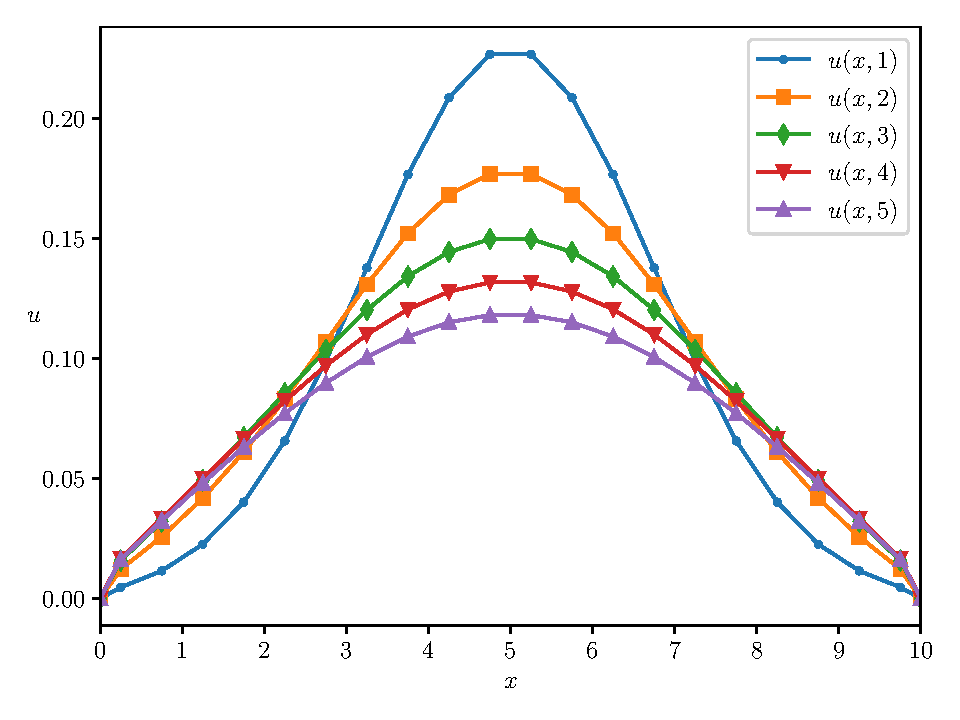
\includegraphics[width=0.8\hsize]{kadai1/1.pdf}
                \caption{オイラー陽解法を用いてDirichlet境界条件のもとで解いた解}
                \label{fig:euler_dirichlet}
            \end{figure}

        \subsubsection{オイラー陽解法、Neumann境界条件}
            オイラー陽解法を用いて、Neumann境界条件$J_L = J_R = 0$のもとで解く。
            定数は、$\Delta t = 0.01, \Delta x = 0.5, N = 20$とした。
            作成したソースコードをコード\ref{src:euler_neumann}に示す。
            \begin{lstlisting}[caption=オイラー陽解法を用いてNeumann境界条件のもとで解くソースコード, label=src:euler_neumann]
#include <iomanip>
#include <iterator>

#include "solver.h"


class EulerSolverWithNeumannCondition: Solver {
private:
    double JL, JR;

    void set_condition_values() override {
        Solver::u[0] = Solver::u[1] - this->JL * Solver::dx;
        Solver::u[Solver::N + 1] = Solver::u[Solver::N] + this->JR * Solver::dx;
    }

public:
    EulerSolverWithNeumannCondition(
        const double dt,
        const double dx,
        const double N,

        const double (*u0)(const double),
        const double JL,
        const double JR
    ): Solver(dt, dx, N) {
        this->JL = JL;
        this->JR = JR;

        this->set_initial_values(u0);
    }

    void solve(const double t_end) override {
        for (int n = 1; n * Solver::dt <= t_end; n++) {
            std::vector<double> u_;
            std::copy(Solver::u.begin(), Solver::u.end(), std::back_inserter(u_));

            for (int i = 1; i <= Solver::N; i++) {
                Solver::u[i] += (u_[i - 1] - 2 * u_[i] + u_[i + 1]) * Solver::dt / Solver::dx / Solver::dx;
            }
            this->set_condition_values();
            
            Solver::print_u(n * Solver::dt);
        }
    }
};


int main() {
    std::cout << std::fixed << std::setprecision(16);

    EulerSolverWithNeumannCondition solver = EulerSolverWithNeumannCondition(0.01, 0.5, 20, u0, 0, 0);
    solver.solve(5);
}\end{lstlisting}

            $t = 1, 2, 3, 4, 5$における数値解を表\ref{tab:euler_neumann}, 図\ref{fig:euler_neumann}にまとめる。
            \begin{table}[h]
                \centering
                \caption{オイラー陽解法を用いてNeumann境界条件のもとで解いた解}
                \label{tab:euler_neumann}
                \begin{tabular}{crrrrcrrrr}
                    \hline
                    $x$ & $u(x, 1)$ & $u(x, 2)$ & $u(x, 3)$ & $u(x, 4)$ & $u(x, 5)$
                    \\
                    \hline
                    \hline
                    0.25 & 0.008510 & 0.030667 & 0.051446 & 0.066829 & 0.077513 \\
                    0.75 & 0.013120 & 0.036405 & 0.055969 & 0.070027 & 0.079704 \\
                    1.25 & 0.023271 & 0.047708 & 0.064661 & 0.076128 & 0.083875 \\
                    1.75 & 0.040421 & 0.064112 & 0.076811 & 0.084566 & 0.089624 \\
                    2.25 & 0.065748 & 0.084665 & 0.091372 & 0.094545 & 0.096395 \\
                    2.75 & 0.099060 & 0.107780 & 0.107008 & 0.105107 & 0.103530 \\
                    3.25 & 0.137792 & 0.131219 & 0.122188 & 0.115219 & 0.110330 \\
                    3.75 & 0.176682 & 0.152291 & 0.135339 & 0.123872 & 0.116125 \\
                    4.25 & 0.208638 & 0.168264 & 0.145032 & 0.130188 & 0.120342 \\
                    4.75 & 0.226757 & 0.176888 & 0.150174 & 0.133518 & 0.122561 \\
                    5.25 & 0.226757 & 0.176888 & 0.150174 & 0.133518 & 0.122561 \\
                    5.75 & 0.208638 & 0.168264 & 0.145032 & 0.130188 & 0.120342 \\
                    6.25 & 0.176682 & 0.152291 & 0.135339 & 0.123872 & 0.116125 \\
                    6.75 & 0.137792 & 0.131219 & 0.122188 & 0.115219 & 0.110330 \\
                    7.25 & 0.099060 & 0.107780 & 0.107008 & 0.105107 & 0.103530 \\
                    7.75 & 0.065748 & 0.084665 & 0.091372 & 0.094545 & 0.096395 \\
                    8.25 & 0.040421 & 0.064112 & 0.076811 & 0.084566 & 0.089624 \\
                    8.75 & 0.023271 & 0.047708 & 0.064661 & 0.076128 & 0.083875 \\
                    9.25 & 0.013120 & 0.036405 & 0.055969 & 0.070027 & 0.079704 \\
                    9.75 & 0.008510 & 0.030667 & 0.051446 & 0.066829 & 0.077513 \\
                    \hline																	
                \end{tabular}
            \end{table}
            \begin{figure}[h]
                \centering
                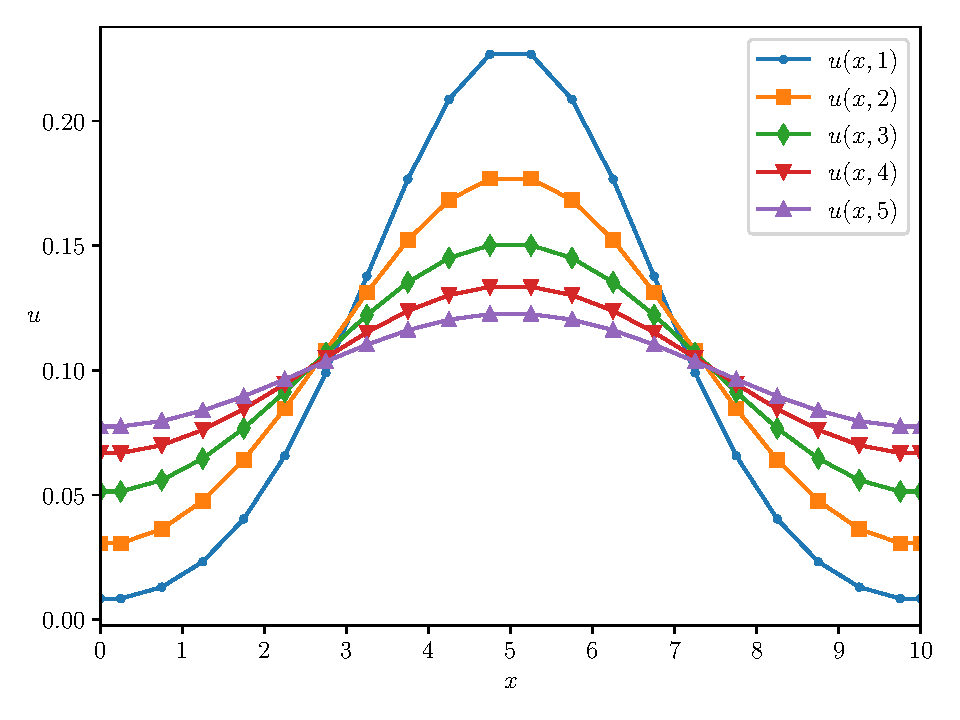
\includegraphics[width=0.8\hsize]{kadai1/2.pdf}
                \caption{オイラー陽解法を用いてNeumann境界条件のもとで解いた解}
                \label{fig:euler_neumann}
            \end{figure}

        \subsubsection{クランク-ニコルソン法、Dirichlet境界条件}
            オイラー陽解法を用いて、Dirichlet境界条件$u_L = u_R = 0$のもとで解く。
            定数は、$\Delta t = 0.01, \Delta x = 0.05, N = 200$とした。
            作成したソースコードをコード\ref{src:crank_dirichlet}に示す。
            \begin{lstlisting}[caption=クランク-ニコルソン法を用いてDirichlet境界条件のもとで解くソースコード, label=src:crank_dirichlet]
#include <iomanip>

#include "solver.h"


class CrankSolverWithDirichletCondition: Solver {
private:
    double c, uL, uR;

    void set_condition_values() override {
        Solver::u[0] = this->uL;
        Solver::u[Solver::N + 1] = this->uR;
    }

    const std::vector<std::vector<double>> calculate_A() {
        std::vector<std::vector<double>> A(Solver::N + 2, std::vector<double>(Solver::N + 2, 0));
        for (int i = 1; i <= Solver::N; i++) {
            A[i][i - 1] = -this->c / 2.0;
            A[i][i] = 1 + this->c;
            A[i][i + 1] = -this->c / 2.0;
        }

        return A;
    }

    const std::pair<std::vector<double>, std::vector<double>> LU_decomposition(
        const std::vector<std::vector<double>> A
    ) {
        std::vector<double> alpha(N + 1, 0), beta(N + 1, 0);
        for (int i = 1; i <= Solver::N; i++) {
            alpha[i] = A[i][i] - A[i][i - 1] * beta[i - 1];
            beta[i] = A[i][i + 1] / alpha[i];
        }

        return std::make_pair(alpha, beta);
    }

    const std::vector<double> calculate_z(
        const std::vector<double> alpha,
        const std::vector<double> beta
    ) {
        std::vector<double> z(N + 1);
        z[1] = (1 - this->c) * Solver::u[1] + this->c * this->uL + this->c / 2.0 * Solver::u[2];
        for (int i = 2; i <= Solver::N - 1; i++) {
            z[i] = (1 - this->c) * Solver::u[i] + this->c / 2.0 * (Solver::u[i - 1] + Solver::u[i + 1]);
        }
        z[N] = (1 - this->c) * Solver::u[N] + this->c * this->uR + this->c / 2.0 * Solver::u[N - 1];

        return z;
    }

    const std::vector<double> calculate_y(
        const std::vector<double> alpha,
        const std::vector<std::vector<double>> A,
        const std::vector<double> z
    ) {
        std::vector<double> y(N + 1, 0);
        for (int i = 1; i <= Solver::N; i++) {
            y[i] = (z[i] - A[i][i - 1] * y[i - 1]) / alpha[i];
        }

        return y;
    }

    const std::vector<double> calculate_x(
        const std::vector<double> beta,
        const std::vector<double> y
    ) {
        std::vector<double> x(N + 2, 0);
        for (int i = N; i >= 1; i--) {
            x[i] = y[i] - beta[i] * x[i + 1];
        }

        return x;
    }

public:
    CrankSolverWithDirichletCondition(
        const double dt,
        const double dx,
        const double N,

        const double (*u0)(const double),
        const double uL,
        const double uR
    ): Solver(dt, dx, N) {
        c = Solver::dt / Solver::dx / Solver::dx;

        this->uL = uL;
        this->uR = uR;

        this->set_initial_values(u0);
    }

    void solve(const double t_end) override {
        const std::vector<std::vector<double>> A = this->calculate_A();

        std::vector<double> alpha, beta;
        std::tie(alpha, beta) = this->LU_decomposition(A);

        for (int n = 1; n * Solver::dt <= t_end; n++) {
            const std::vector<double> z = this->calculate_z(alpha, beta);
            const std::vector<double> y = this->calculate_y(alpha, A, z);
            const std::vector<double> x = this->calculate_x(beta, y);

            for (int i = 1; i <= N; i++) {
                Solver::u[i] = x[i];
            }

            this->set_condition_values();
            
            Solver::print_u(n * Solver::dt);
        }
    }
};


int main() {
    std::cout << std::fixed << std::setprecision(16);

    CrankSolverWithDirichletCondition solver = CrankSolverWithDirichletCondition(0.01, 0.05, 200, u0, 0, 0);
    solver.solve(5);
}\end{lstlisting}

            $t = 1, 2, 3, 4, 5$における数値解を表\ref{tab:crank_dirichlet}, 図\ref{fig:crank_dirichlet}にまとめる。
            \begin{table}[h]
                \caption{クランク-ニコルソン法を用いてDirichlet境界条件のもとで解いた解}
                \label{tab:crank_dirichlet}
                \centering
                \begin{tabular}{ccccccc}
                    \hline
                    $x$ & $u(x, 1)$ & $u(x, 2)$ & $u(x, 3)$ & $u(x, 4)$ & $u(x, 5)$
                    \\
                    \hline
                    \hline
                    0.025 & 0.000574 & 0.001436 & 0.001783 & 0.001826 & 0.001743 \\
                    0.075 & 0.001151 & 0.002873 & 0.003566 & 0.003651 & 0.003486 \\
                    0.125 & 0.001734 & 0.004313 & 0.005350 & 0.005476 & 0.005228 \\
                    0.175 & 0.002324 & 0.005757 & 0.007135 & 0.007301 & 0.006970 \\
                    0.225 & 0.002924 & 0.007207 & 0.008921 & 0.009126 & 0.008710 \\
                    0.275 & 0.003537 & 0.008665 & 0.010710 & 0.010950 & 0.010449 \\
                    0.325 & 0.004166 & 0.010131 & 0.012500 & 0.012773 & 0.012186 \\
                    0.375 & 0.004813 & 0.011607 & 0.014294 & 0.014596 & 0.013921 \\
                    0.425 & 0.005481 & 0.013095 & 0.016090 & 0.016418 & 0.015654 \\
                    0.475 & 0.006172 & 0.014596 & 0.017889 & 0.018239 & 0.017385 \\
                    \vdots & \vdots & \vdots & \vdots & \vdots & \vdots \vspace{1mm} \\
                    4.775 & 0.228385 & 0.177493 & 0.150007 & 0.131605 & 0.117522 \\
                    4.825 & 0.229148 & 0.177849 & 0.150226 & 0.131764 & 0.117649 \\
                    4.875 & 0.229721 & 0.178116 & 0.150391 & 0.131883 & 0.117744 \\
                    4.925 & 0.230105 & 0.178295 & 0.150501 & 0.131962 & 0.117808 \\
                    4.975 & 0.230296 & 0.178384 & 0.150556 & 0.132002 & 0.117840 \\
                    5.025 & 0.230296 & 0.178384 & 0.150556 & 0.132002 & 0.117840 \\
                    5.075 & 0.230105 & 0.178295 & 0.150501 & 0.131962 & 0.117808 \\
                    5.125 & 0.229721 & 0.178116 & 0.150391 & 0.131883 & 0.117744 \\
                    5.175 & 0.229148 & 0.177849 & 0.150226 & 0.131764 & 0.117649 \\
                    5.225 & 0.228385 & 0.177493 & 0.150007 & 0.131605 & 0.117522 \\
                    \vdots & \vdots & \vdots & \vdots & \vdots & \vdots \vspace{1mm} \\
                    9.525 & 0.006172 & 0.014596 & 0.017889 & 0.018239 & 0.017385 \\
                    9.575 & 0.005481 & 0.013095 & 0.016090 & 0.016418 & 0.015654 \\
                    9.625 & 0.004813 & 0.011607 & 0.014294 & 0.014596 & 0.013921 \\
                    9.675 & 0.004166 & 0.010131 & 0.012500 & 0.012773 & 0.012186 \\
                    9.725 & 0.003537 & 0.008665 & 0.010710 & 0.010950 & 0.010449 \\
                    9.775 & 0.002924 & 0.007207 & 0.008921 & 0.009126 & 0.008710 \\
                    9.825 & 0.002324 & 0.005757 & 0.007135 & 0.007301 & 0.006970 \\
                    9.875 & 0.001734 & 0.004313 & 0.005350 & 0.005476 & 0.005228 \\
                    9.925 & 0.001151 & 0.002873 & 0.003566 & 0.003651 & 0.003486 \\
                    9.975 & 0.000574 & 0.001436 & 0.001783 & 0.001826 & 0.001743 \\
                    \hline																	
                \end{tabular}
            \end{table}
            \begin{figure}[h]
                \centering
                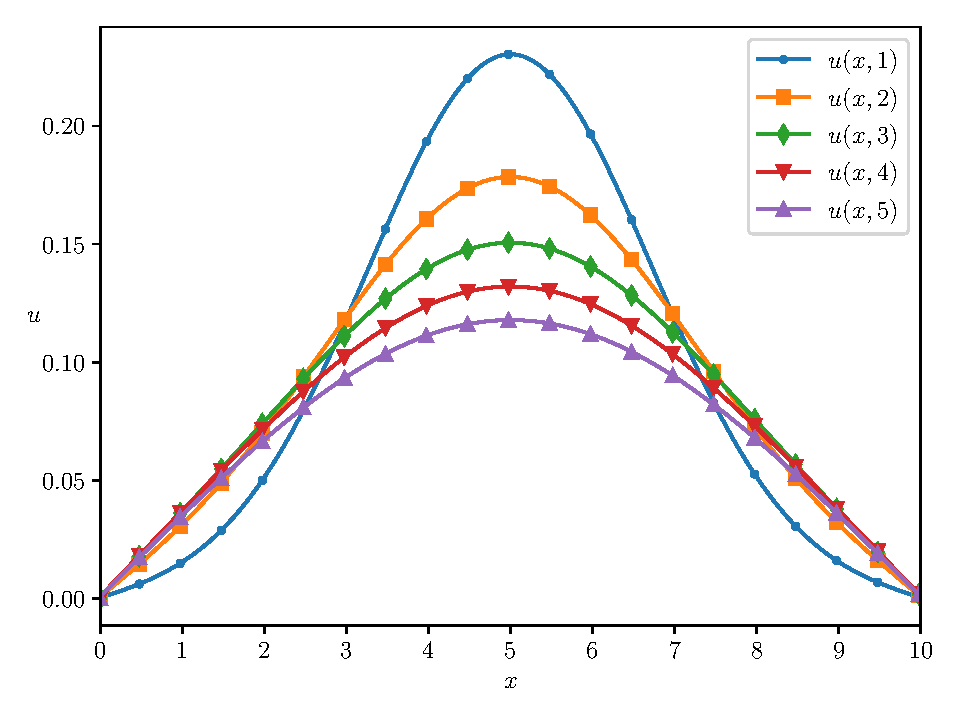
\includegraphics[width=0.8\hsize]{kadai1/3.pdf}
                \caption{クランク-ニコルソン法を用いてDirichlet境界条件のもとで解いた解}
                \label{fig:crank_dirichlet}
            \end{figure}

        \subsubsection{クランク-ニコルソン法、Neumann境界条件}
            オイラー陽解法を用いて、Neumann境界条件$J_L = J_R = 0$のもとで解く。
            定数は、$\Delta t = 0.01, \Delta x = 0.05, N = 200$とした。
            作成したソースコードをコード\ref{src:crank_neumann}に示す。
            \begin{lstlisting}[caption=クランク-ニコルソン法を用いてNeumann境界条件のもとで解くソースコード, label=src:crank_neumann]
#include <iomanip>

#include "solver.h"


class CrankSolverWithNeumannCondition: Solver {
private:
    double c, JL, JR;

    void set_condition_values() override {
        Solver::u[0] = Solver::u[1] - this->JL * Solver::dx;
        Solver::u[Solver::N + 1] = Solver::u[Solver::N] + this->JR * Solver::dx;
    }

    const std::vector<std::vector<double>> calculate_A() {
        std::vector<std::vector<double>> A(Solver::N + 2, std::vector<double>(Solver::N + 2, 0));
        for (int i = 1; i <= Solver::N; i++) {
            A[i][i - 1] = -this->c / 2.0;
            A[i][i] = 1 + this->c;
            A[i][i + 1] = -this->c / 2.0;
        }
        A[1][1] -= this->c / 2.0;
        A[N][N] -= this->c / 2.0;

        return A;
    }

    const std::pair<std::vector<double>, std::vector<double>> LU_decomposition(
        const std::vector<std::vector<double>> A
    ) {
        std::vector<double> alpha(N + 1, 0), beta(N + 1, 0);
        for (int i = 1; i <= Solver::N; i++) {
            alpha[i] = A[i][i] - A[i][i - 1] * beta[i - 1];
            beta[i] = A[i][i + 1] / alpha[i];
        }

        return std::make_pair(alpha, beta);
    }

    const std::vector<double> calculate_z(
        const std::vector<double> alpha,
        const std::vector<double> beta
    ) {
        std::vector<double> z(N + 1);
        z[1] = (1 - this->c / 2.0) * Solver::u[1] - this->c * this->JL * Solver::dx + this->c / 2.0 * Solver::u[2];
        for (int i = 2; i <= Solver::N - 1; i++) {
            z[i] = (1 - this->c) * Solver::u[i] + this->c / 2.0 * (Solver::u[i - 1] + Solver::u[i + 1]);
        }
        z[N] = (1 - this->c / 2.0) * Solver::u[N] + this->c * this->JR * Solver::dx + this->c / 2.0 * Solver::u[N - 1];

        return z;
    }

    const std::vector<double> calculate_y(
        const std::vector<double> alpha,
        const std::vector<std::vector<double>> A,
        const std::vector<double> z
    ) {
        std::vector<double> y(N + 1, 0);
        for (int i = 1; i <= Solver::N; i++) {
            y[i] = (z[i] - A[i][i - 1] * y[i - 1]) / alpha[i];
        }

        return y;
    }

    const std::vector<double> calculate_x(
        const std::vector<double> beta,
        const std::vector<double> y
    ) {
        std::vector<double> x(N + 2, 0);
        for (int i = N; i >= 1; i--) {
            x[i] = y[i] - beta[i] * x[i + 1];
        }

        return x;
    }

public:
    CrankSolverWithNeumannCondition(
        const double dt,
        const double dx,
        const double N,

        const double (*u0)(const double),
        const double JL,
        const double JR
    ): Solver(dt, dx, N) {
        c = Solver::dt / Solver::dx / Solver::dx;

        this->JL = JL;
        this->JR = JR;

        this->set_initial_values(u0);
    }

    void solve(const double t_end) override {
        const std::vector<std::vector<double>> A = this->calculate_A();

        std::vector<double> alpha, beta;
        std::tie(alpha, beta) = this->LU_decomposition(A);

        for (int n = 1; n * Solver::dt <= t_end; n++) {
            const std::vector<double> z = this->calculate_z(alpha, beta);
            const std::vector<double> y = this->calculate_y(alpha, A, z);
            const std::vector<double> x = this->calculate_x(beta, y);

            for (int i = 1; i <= N; i++) {
                Solver::u[i] = x[i];
            }

            this->set_condition_values();
            
            Solver::print_u(n * Solver::dt);
        }
    }
};


int main() {
    std::cout << std::fixed << std::setprecision(16);

    CrankSolverWithNeumannCondition solver = CrankSolverWithNeumannCondition(0.01, 0.05, 200, u0, 0, 0);
    solver.solve(5);
}\end{lstlisting}

            $t = 1, 2, 3, 4, 5$における数値解を表\ref{tab:crank_neumann}, 図\ref{fig:crank_neumann}にまとめる。
            \begin{table}[h]
                \centering
                \caption{クランク-ニコルソン法を用いてNeumann境界条件のもとで解いた解}
                \label{tab:crank_neumann}
                \begin{tabular}{ccccccc}
                    \hline
                    $x$ & $u(x, 1)$ & $u(x, 2)$ & $u(x, 3)$ & $u(x, 4)$ & $u(x, 5)$
                    \\
                    \hline
                    \hline
                    0.025 & 0.007156 & 0.029303 & 0.050575 & 0.066323 & 0.077230 \\
                    0.075 & 0.007200 & 0.029362 & 0.050621 & 0.066356 & 0.077253 \\
                    0.125 & 0.007287 & 0.029479 & 0.050714 & 0.066421 & 0.077297 \\
                    0.175 & 0.007419 & 0.029655 & 0.050853 & 0.066520 & 0.077364 \\
                    0.225 & 0.007595 & 0.029889 & 0.051038 & 0.066650 & 0.077454 \\
                    0.275 & 0.007815 & 0.030181 & 0.051270 & 0.066813 & 0.077565 \\
                    0.325 & 0.008081 & 0.030532 & 0.051547 & 0.067009 & 0.077698 \\
                    0.375 & 0.008393 & 0.030941 & 0.051870 & 0.067236 & 0.077854 \\
                    0.425 & 0.008751 & 0.031409 & 0.052238 & 0.067496 & 0.078031 \\
                    0.475 & 0.009158 & 0.031934 & 0.052652 & 0.067787 & 0.078230 \\
                    \vdots & \vdots & \vdots & \vdots & \vdots & \vdots \vspace{1mm} \\
                    4.775 & 0.228385 & 0.177527 & 0.150491 & 0.133665 & 0.122611 \\
                    4.825 & 0.229148 & 0.177881 & 0.150701 & 0.133801 & 0.122702 \\
                    4.875 & 0.229721 & 0.178148 & 0.150859 & 0.133903 & 0.122770 \\
                    4.925 & 0.230105 & 0.178326 & 0.150964 & 0.133971 & 0.122815 \\
                    4.975 & 0.230296 & 0.178415 & 0.151017 & 0.134005 & 0.122837 \\
                    5.025 & 0.230296 & 0.178415 & 0.151017 & 0.134005 & 0.122837 \\
                    5.075 & 0.230105 & 0.178326 & 0.150964 & 0.133971 & 0.122815 \\
                    5.125 & 0.229721 & 0.178148 & 0.150859 & 0.133903 & 0.122770 \\
                    5.175 & 0.229148 & 0.177881 & 0.150701 & 0.133801 & 0.122702 \\
                    5.225 & 0.228385 & 0.177527 & 0.150491 & 0.133665 & 0.122611 \\
                    \vdots & \vdots & \vdots & \vdots & \vdots & \vdots \vspace{1mm} \\
                    9.525 & 0.009158 & 0.031934 & 0.052652 & 0.067787 & 0.078230 \\
                    9.575 & 0.008751 & 0.031409 & 0.052238 & 0.067496 & 0.078031 \\
                    9.625 & 0.008393 & 0.030941 & 0.051870 & 0.067236 & 0.077854 \\
                    9.675 & 0.008081 & 0.030532 & 0.051547 & 0.067009 & 0.077698 \\
                    9.725 & 0.007815 & 0.030181 & 0.051270 & 0.066813 & 0.077565 \\
                    9.775 & 0.007595 & 0.029889 & 0.051038 & 0.066650 & 0.077454 \\
                    9.825 & 0.007419 & 0.029655 & 0.050853 & 0.066520 & 0.077364 \\
                    9.875 & 0.007287 & 0.029479 & 0.050714 & 0.066421 & 0.077297 \\
                    9.925 & 0.007200 & 0.029362 & 0.050621 & 0.066356 & 0.077253 \\
                    9.975 & 0.007156 & 0.029303 & 0.050575 & 0.066323 & 0.077230 \\
                    \hline																	
                    \end{tabular}
            \end{table}
            \begin{figure}[h]
                \centering
                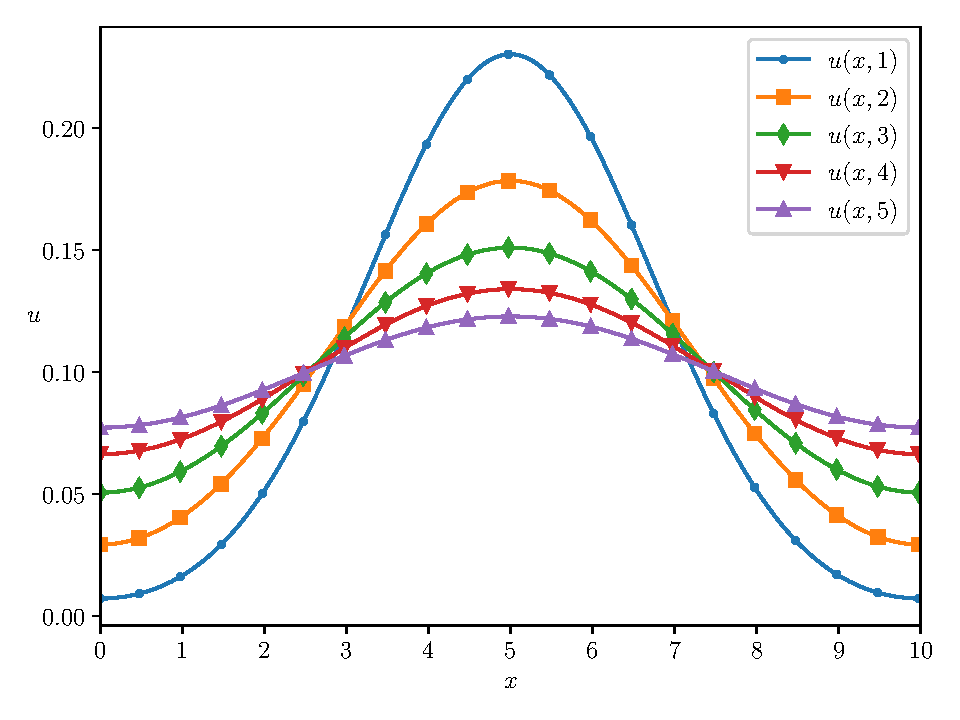
\includegraphics[width=0.8\hsize]{kadai1/4.pdf}
                \caption{クランク-ニコルソン法を用いてNeumann境界条件のもとで解いた解}
                \label{fig:crank_neumann}
            \end{figure}

    \subsection{課題2 Fisher方程式}
        式(\ref{equ:diffusion})に非線形項$f(u) = u(1-u)$を加えた式を
        Fisher方程式と呼ぶ。
        \begin{equation}
            \frac{\partial u}{\partial t} = u(1 - u) + \frac{\partial^2u}{\partial x^2} \label{equ:fisher}
        \end{equation}

        これは、式(\ref{equ:fisher_euler})に示すオイラー陽解法で解くことができる。
        \begin{eqnarray}
            \frac{u_j^{n + 1} - u_j^n}{\Delta t} &=& f(u_j^n) + \frac{u_{j - 1}^n - 2u_j^n + u_{j + 1}^n}{\Delta x^2} \nonumber \\
            \rightarrow u_j^{n + 1} &=& u_j^n + \Delta t\left\{f(u_j^n) + \frac{u_{j - 1}^n - 2u_j^n + u_{j + 1}^n}{\Delta x^2} \label{equ:fisher_euler}\right\}
        \end{eqnarray}

        式(\ref{equ:fisher})を、
        $x\in[0, L = 200]$について、初期条件
        \begin{equation*}
            u_0(x) = \displaystyle\frac{1}{(1 + e^{bx - 5})^2} \ (b = 0.25, 0.5, 1)
        \end{equation*}
        のもとで解く。
        境界条件はDirichlet境界条件
        \begin{eqnarray*}
            u(0, t) &=& 1 \\
            u(L, t) &=& 0
        \end{eqnarray*}
        を用い、各定数は
        $\Delta t = 0.001, \Delta x = 0.05, N = 4000$とした。

        \subsubsection{解法}
            作成したソースコードをコード\ref{src:fisher}, \ref{src:fisher_u0}に示す。
            なお、コード\ref{src:solver}に示したsolver.hを使用している。
            \begin{lstlisting}[caption=式(\ref{equ:fisher_euler})の実装, label=src:fisher]
#include <iomanip>
#include <iterator>

#include "solver.h"


double b;


class EulerSolverWithDirichletCondition: Solver {
private:
    double uL, uR;

    void set_condition_values() override {
        Solver::u[0] = this->uL;
        Solver::u[Solver::N + 1] = this->uR;
    }

public:
    EulerSolverWithDirichletCondition(
        const double dt,
        const double dx,
        const double N,

        const double (*u0)(const double),
        const double uL,
        const double uR
    ): Solver(dt, dx, N) {
        this->uL = uL;
        this->uR = uR;

        this->set_initial_values(u0);
    }

    void solve(const double t_end) override {
        for (int n = 1; n * Solver::dt <= t_end; n++) {
            std::vector<double> u_;
            std::copy(Solver::u.begin(), Solver::u.end(), std::back_inserter(u_));

            for (int i = 1; i <= Solver::N; i++) {
                Solver::u[i] += Solver::dt * (u_[i] * (1 - u_[i]) + (u_[i - 1] - 2 * u_[i] + u_[i + 1]) / Solver::dx / Solver::dx);
            }
            this->set_condition_values();
            
            Solver::print_u(n * Solver::dt);
        }
    }
};


int main(const int argc, const char *argv[]) {
    if (argc != 2) {
        return EXIT_FAILURE;
    }
    b = atof(argv[1]);
    
    std::cout << std::fixed << std::setprecision(16);

    EulerSolverWithDirichletCondition solver = EulerSolverWithDirichletCondition(0.001, 0.05, 4000, u0, 1, 0);
    solver.solve(40);
}\end{lstlisting}
            \begin{lstlisting}[caption=$u_0(x)$の実装, label=src:fisher_u0]
#include <cmath>

const double u0(const double x) {
    return 1.0 / (1.0 + exp(b * x - 5.0)) / (1.0 + exp(b * x - 5.0));
}\end{lstlisting}

        \subsubsection{結果}
            $t = 10, 20, 30, 40$数値解を表\ref{tab:fisher25}, \ref{tab:fisher50}, \ref{tab:fisher100},
            図\ref{fig:fisher25}, \ref{fig:fisher50}, \ref{fig:fisher100}にまとめる。
            \begin{table}[h]
                \caption{Fisher方程式の数値解 ($b = 0.25$)}
                \label{tab:fisher25}
                \centering
                \begin{tabular}{ccccccc}
                    \hline
                    $x$ & $u(x, 10)$ & $u(x, 20)$ & $u(x, 30)$ & $u(x, 40)$
                    \\
                    \hline
                    \hline
                    0.025 & 1.000000 & 1.000000 & 1.000000 & 1.000000 \\
                    0.075 & 1.000000 & 1.000000 & 1.000000 & 1.000000 \\
                    0.125 & 1.000000 & 1.000000 & 1.000000 & 1.000000 \\
                    0.175 & 1.000000 & 1.000000 & 1.000000 & 1.000000 \\
                    0.225 & 1.000000 & 1.000000 & 1.000000 & 1.000000 \\
                    0.275 & 1.000000 & 1.000000 & 1.000000 & 1.000000 \\
                    0.325 & 1.000000 & 1.000000 & 1.000000 & 1.000000 \\
                    0.375 & 1.000000 & 1.000000 & 1.000000 & 1.000000 \\
                    0.425 & 1.000000 & 1.000000 & 1.000000 & 1.000000 \\
                    0.475 & 1.000000 & 1.000000 & 1.000000 & 1.000000 \\
                    \vdots & \vdots & \vdots & \vdots & \vdots \vspace{1mm} \\
                    99.775 & 0.000000 & 0.000000 & 0.077225 & 0.999005 \\
                    99.825 & 0.000000 & 0.000000 & 0.075562 & 0.998987 \\
                    99.875 & 0.000000 & 0.000000 & 0.073930 & 0.998969 \\
                    99.925 & 0.000000 & 0.000000 & 0.072330 & 0.998951 \\
                    99.975 & 0.000000 & 0.000000 & 0.070759 & 0.998932 \\
                    100.025 & 0.000000 & 0.000000 & 0.069219 & 0.998914 \\
                    100.075 & 0.000000 & 0.000000 & 0.067708 & 0.998894 \\
                    100.125 & 0.000000 & 0.000000 & 0.066227 & 0.998875 \\
                    100.175 & 0.000000 & 0.000000 & 0.064774 & 0.998855 \\
                    100.225 & 0.000000 & 0.000000 & 0.063350 & 0.998835 \\
                    \vdots & \vdots & \vdots & \vdots & \vdots \vspace{1mm} \\
                    199.525 & 0.000000 & 0.000000 & 0.000000 & 0.000000 \\
                    199.575 & 0.000000 & 0.000000 & 0.000000 & 0.000000 \\
                    199.625 & 0.000000 & 0.000000 & 0.000000 & 0.000000 \\
                    199.675 & 0.000000 & 0.000000 & 0.000000 & 0.000000 \\
                    199.725 & 0.000000 & 0.000000 & 0.000000 & 0.000000 \\
                    199.775 & 0.000000 & 0.000000 & 0.000000 & 0.000000 \\
                    199.825 & 0.000000 & 0.000000 & 0.000000 & 0.000000 \\
                    199.875 & 0.000000 & 0.000000 & 0.000000 & 0.000000 \\
                    199.925 & 0.000000 & 0.000000 & 0.000000 & 0.000000 \\
                    199.975 & 0.000000 & 0.000000 & 0.000000 & 0.000000 \\
                    \hline																	
                \end{tabular}
            \end{table}
            \begin{table}[h]
                \caption{Fisher方程式の数値解 ($b = 0.5$)}
                \label{tab:fisher50}
                \centering
                \begin{tabular}{ccccccc}
                    \hline
                    $x$ & $u(x, 10)$ & $u(x, 20)$ & $u(x, 30)$ & $u(x, 40)$
                    \\
                    \hline
                    \hline
                    0.025 & 1.000000 & 1.000000 & 1.000000 & 1.000000 \\
                    0.075 & 0.999999 & 1.000000 & 1.000000 & 1.000000 \\
                    0.125 & 0.999999 & 1.000000 & 1.000000 & 1.000000 \\
                    0.175 & 0.999999 & 1.000000 & 1.000000 & 1.000000 \\
                    0.225 & 0.999998 & 1.000000 & 1.000000 & 1.000000 \\
                    0.275 & 0.999998 & 1.000000 & 1.000000 & 1.000000 \\
                    0.325 & 0.999998 & 1.000000 & 1.000000 & 1.000000 \\
                    0.375 & 0.999998 & 1.000000 & 1.000000 & 1.000000 \\
                    0.425 & 0.999997 & 1.000000 & 1.000000 & 1.000000 \\
                    0.475 & 0.999997 & 1.000000 & 1.000000 & 1.000000 \\
                    \vdots & \vdots & \vdots & \vdots & \vdots \vspace{1mm} \\
                    99.775 & 0.000000 & 0.000000 & 0.000000 & 0.000037 \\
                    99.825 & 0.000000 & 0.000000 & 0.000000 & 0.000036 \\
                    99.875 & 0.000000 & 0.000000 & 0.000000 & 0.000034 \\
                    99.925 & 0.000000 & 0.000000 & 0.000000 & 0.000033 \\
                    99.975 & 0.000000 & 0.000000 & 0.000000 & 0.000031 \\
                    100.025 & 0.000000 & 0.000000 & 0.000000 & 0.000030 \\
                    100.075 & 0.000000 & 0.000000 & 0.000000 & 0.000028 \\
                    100.125 & 0.000000 & 0.000000 & 0.000000 & 0.000027 \\
                    100.175 & 0.000000 & 0.000000 & 0.000000 & 0.000026 \\
                    100.225 & 0.000000 & 0.000000 & 0.000000 & 0.000025 \\
                    \vdots & \vdots & \vdots & \vdots & \vdots \vspace{1mm} \\
                    199.525 & 0.000000 & 0.000000 & 0.000000 & 0.000000 \\
                    199.575 & 0.000000 & 0.000000 & 0.000000 & 0.000000 \\
                    199.625 & 0.000000 & 0.000000 & 0.000000 & 0.000000 \\
                    199.675 & 0.000000 & 0.000000 & 0.000000 & 0.000000 \\
                    199.725 & 0.000000 & 0.000000 & 0.000000 & 0.000000 \\
                    199.775 & 0.000000 & 0.000000 & 0.000000 & 0.000000 \\
                    199.825 & 0.000000 & 0.000000 & 0.000000 & 0.000000 \\
                    199.875 & 0.000000 & 0.000000 & 0.000000 & 0.000000 \\
                    199.925 & 0.000000 & 0.000000 & 0.000000 & 0.000000 \\
                    199.975 & 0.000000 & 0.000000 & 0.000000 & 0.000000 \\
                    \hline																	
                \end{tabular}
            \end{table}
            \begin{table}[h]
                \caption{Fisher方程式の数値解 ($b = 1$)}
                \label{tab:fisher100}
                \centering
                \begin{tabular}{ccccccc}
                    \hline
                    $x$ & $u(x, 10)$ & $u(x, 20)$ & $u(x, 30)$ & $u(x, 40)$
                    \\
                    \hline
                    \hline
                    0.025 & 0.999996 & 1.000000 & 1.000000 & 1.000000 \\
                    0.075 & 0.999992 & 1.000000 & 1.000000 & 1.000000 \\
                    0.125 & 0.999988 & 1.000000 & 1.000000 & 1.000000 \\
                    0.175 & 0.999984 & 1.000000 & 1.000000 & 1.000000 \\
                    0.225 & 0.999981 & 1.000000 & 1.000000 & 1.000000 \\
                    0.275 & 0.999977 & 1.000000 & 1.000000 & 1.000000 \\
                    0.325 & 0.999973 & 1.000000 & 1.000000 & 1.000000 \\
                    0.375 & 0.999969 & 1.000000 & 1.000000 & 1.000000 \\
                    0.425 & 0.999965 & 1.000000 & 1.000000 & 1.000000 \\
                    0.475 & 0.999961 & 1.000000 & 1.000000 & 1.000000 \\
                    \vdots & \vdots & \vdots & \vdots & \vdots \vspace{1mm} \\
                    99.775 & 0.000000 & 0.000000 & 0.000000 & 0.000000 \\
                    99.825 & 0.000000 & 0.000000 & 0.000000 & 0.000000 \\
                    99.875 & 0.000000 & 0.000000 & 0.000000 & 0.000000 \\
                    99.925 & 0.000000 & 0.000000 & 0.000000 & 0.000000 \\
                    99.975 & 0.000000 & 0.000000 & 0.000000 & 0.000000 \\
                    100.025 & 0.000000 & 0.000000 & 0.000000 & 0.000000 \\
                    100.075 & 0.000000 & 0.000000 & 0.000000 & 0.000000 \\
                    100.125 & 0.000000 & 0.000000 & 0.000000 & 0.000000 \\
                    100.175 & 0.000000 & 0.000000 & 0.000000 & 0.000000 \\
                    100.225 & 0.000000 & 0.000000 & 0.000000 & 0.000000 \\
                    \vdots & \vdots & \vdots & \vdots & \vdots \vspace{1mm} \\
                    199.525 & 0.000000 & 0.000000 & 0.000000 & 0.000000 \\
                    199.575 & 0.000000 & 0.000000 & 0.000000 & 0.000000 \\
                    199.625 & 0.000000 & 0.000000 & 0.000000 & 0.000000 \\
                    199.675 & 0.000000 & 0.000000 & 0.000000 & 0.000000 \\
                    199.725 & 0.000000 & 0.000000 & 0.000000 & 0.000000 \\
                    199.775 & 0.000000 & 0.000000 & 0.000000 & 0.000000 \\
                    199.825 & 0.000000 & 0.000000 & 0.000000 & 0.000000 \\
                    199.875 & 0.000000 & 0.000000 & 0.000000 & 0.000000 \\
                    199.925 & 0.000000 & 0.000000 & 0.000000 & 0.000000 \\
                    199.975 & 0.000000 & 0.000000 & 0.000000 & 0.000000 \\
                    \hline																	
                \end{tabular}
            \end{table}
            \begin{figure}[h]
                \centering
                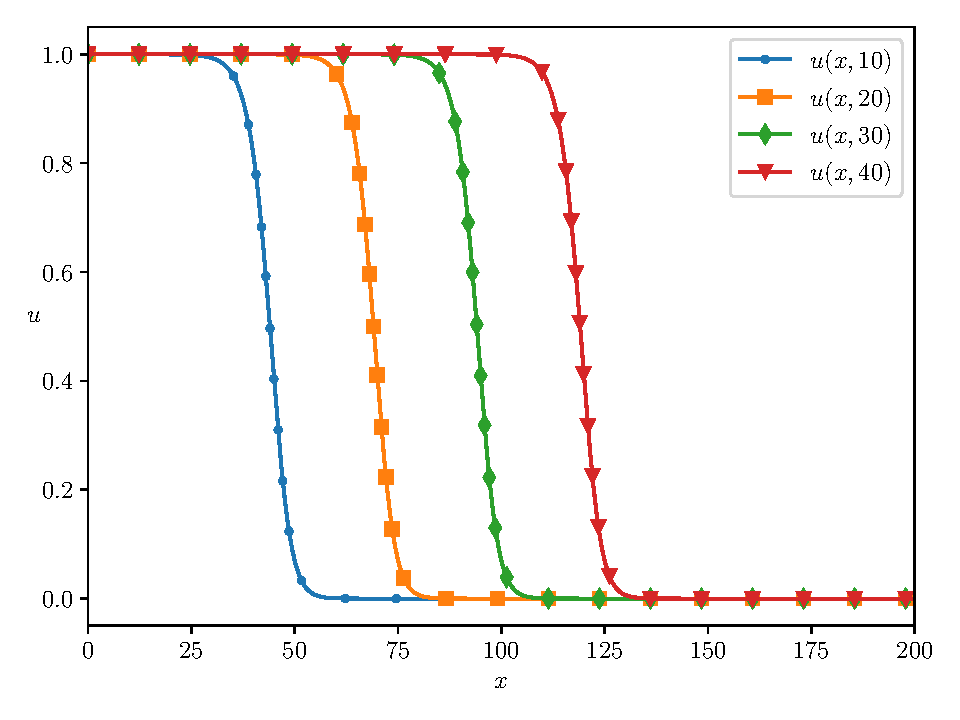
\includegraphics[width=0.8\hsize]{kadai2/25.pdf}
                \caption{Fisher方程式の数値解 ($b = 0.25$)}
                \label{fig:fisher25}
            \end{figure}
            \begin{figure}[h]
                \centering
                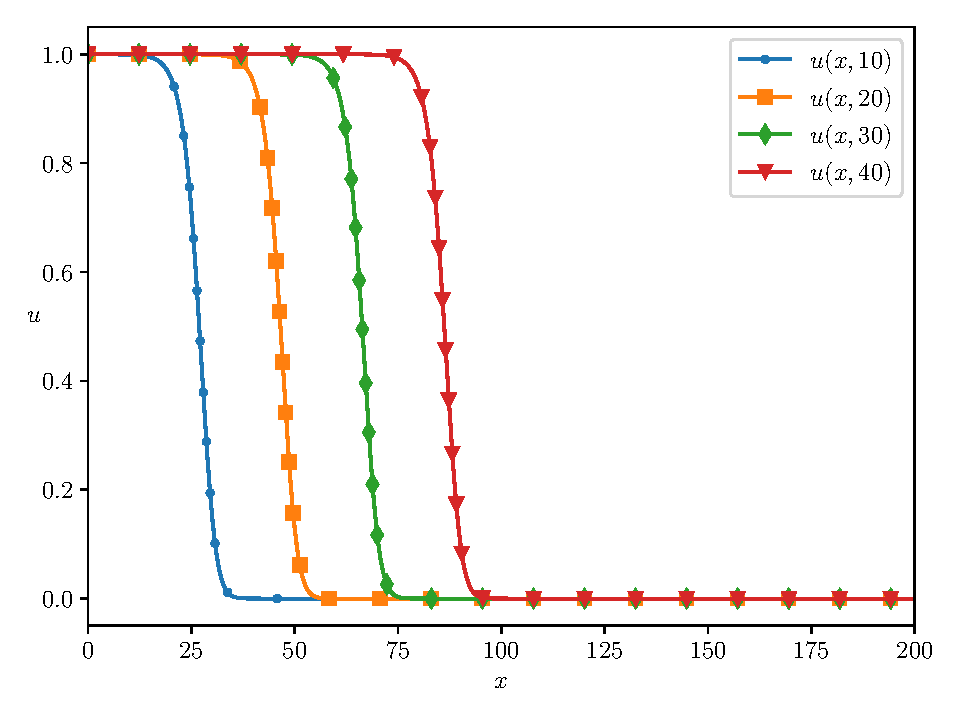
\includegraphics[width=0.8\hsize]{kadai2/50.pdf}
                \caption{Fisher方程式の数値解 ($b = 0.5$)}
                \label{fig:fisher50}
            \end{figure}
            \begin{figure}[h]
                \centering
                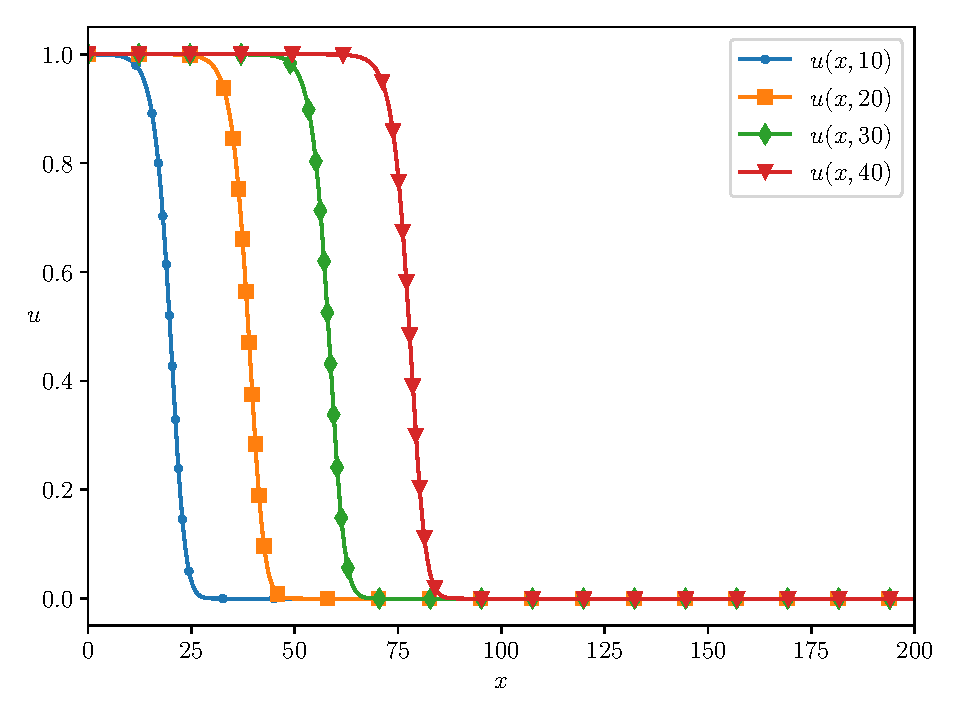
\includegraphics[width=0.8\hsize]{kadai2/100.pdf}
                \caption{Fisher方程式の数値解 ($b = 1$)}
                \label{fig:fisher100}
            \end{figure}

        \subsubsection{考察}
            図\ref{fig:fisher25}, \ref{fig:fisher50}, \ref{fig:fisher100}
            を比較すると、
            $b$が大きくなるにつれ、
            ある時刻で$u$が1から0へと変化する$x$が小さくなっていることがわかる。
            この様子を図\ref{fig:fisher_compare}に示す。
            これは、初期条件$u_0(x)$に現れている特徴でもあるため、
            当然であると言える。
            \begin{figure}[h]
                \centering
                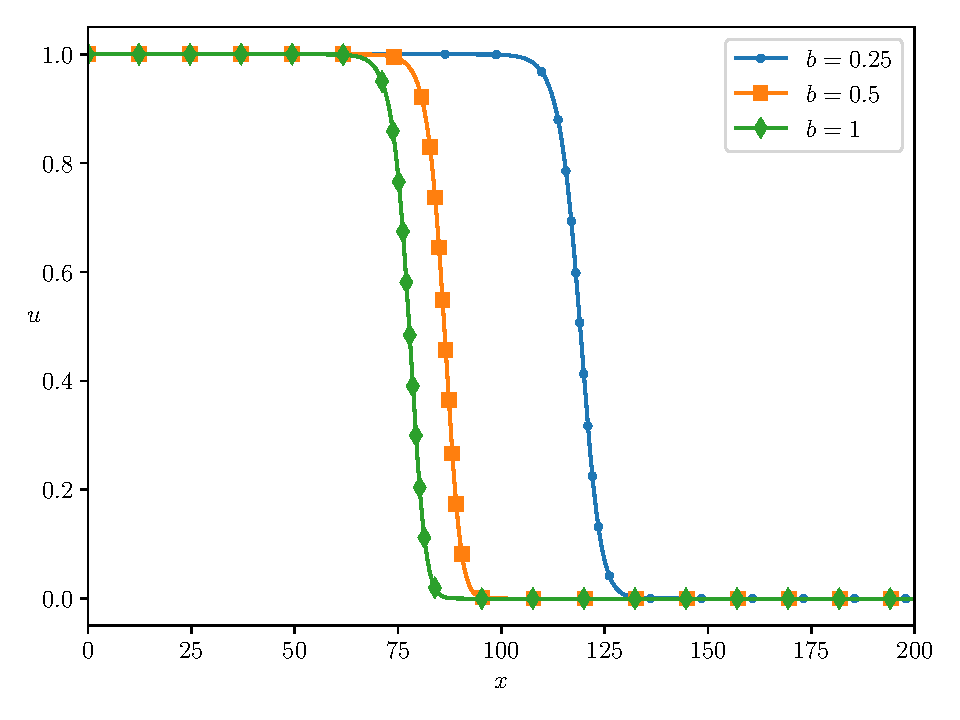
\includegraphics[width=0.8\hsize]{kadai2/compare.pdf}
                \caption{Fisher方程式の数値解の比較 ($t = 40$)}
                \label{fig:fisher_compare}
            \end{figure}

    \subsection{課題3 1次元調和振動子のSchr\"{o}dinger方程式}
        式(\ref{equ:schroedinger})にSchr\"{o}dinger方程式を示す。
        \begin{equation}
            i\hbar\frac{\partial\psi}{\partial t}(x, t) = \left(-\frac{\hbar^2}{2m}\frac{\partial^2}{\partial x^2} + \frac{k}{2}x^2\right)\psi(x, t) \label{equ:schroedinger}
        \end{equation}
        $\psi(x, t)\in\mathbb{C}$を
        $\psi(x, t) = \psi_R(x, t) + i\psi_I(x, t) \ (\psi_R, \psi_I\in\mathbb{R})$
        のように実部と虚部に分解すると、
        式(\ref{equ:schroedinger})は
        \begin{eqnarray*}
            \hbar\frac{\partial\psi_R}{\partial t}(x, t) &=& \left(-\frac{\hbar^2}{2m}\frac{\partial^2}{\partial x^2} + \frac{k}{2}x^2\right)\psi_I(x, t) \\
            -\hbar\frac{\partial\psi_I}{\partial t}(x, t) &=& \left(-\frac{\hbar^2}{2m}\frac{\partial^2}{\partial x^2} + \frac{k}{2}x^2\right)\psi_R(x, t)
        \end{eqnarray*}
        と書き換えられる。
        このとき、粒子の位置の確率密度は
        $\psi_R^2 + \psi_I^2$で示される。

        \subsubsection{数値解法}
            $h=m=k=1$とした方程式
            \begin{eqnarray*}
                \frac{\partial\psi_R}{\partial t} &=& \left(-\frac{1}{2}\frac{\partial^2}{\partial x^2} + \frac{1}{2}x^2\right)\psi_I \\
                -\frac{\partial\psi_I}{\partial t} &=& \left(-\frac{1}{2}\frac{\partial^2}{\partial x^2} + \frac{1}{2}x^2\right)\psi_R
            \end{eqnarray*}
            は次に示すオイラー陽解法を用いて解くことができる。
            \begin{eqnarray*}
                R_j^{n+1} &=& R_j^n + \Delta t\left(-\frac{1}{2}\frac{I_{j-1}^n-2I_j^n+I_{j+1}^n}{\Delta x^2}+\frac{1}{2}x_j^2I_j^n\right) \ \left(\psi_R(x, n\Delta t) \coloneqq \{R_j^n\}\right) \\
                I_j^{n+1} &=& I_j^n - \Delta t\left(-\frac{1}{2}\frac{R_{j-1}^{n+1}-2R_j^{n+1}+R_{j+1}^{n+1}}{\Delta x^2}+\frac{1}{2}x_j^2R_j^{n+1}\right) \ \left(\psi_I(x, n\Delta t) \coloneqq \{I_j^n\}\right) \\
                x_j &\coloneqq& \left(j - \frac{1}{2}\right)\Delta x - \frac{L}{2}
            \end{eqnarray*}
            本実験では周期境界条件
            $\displaystyle\psi\left(\frac{L}{2}, t\right) = \psi\left(-\frac{L}{2}, t\right)$
            を用いて解く。これは、次のように表される。
            \begin{eqnarray*}
                R_0^n = R_N^n&,& R_{N+1}^n = R_1^n \\
                I_0^n = I_N^n&,& I_{N+1}^n = I_1^n
            \end{eqnarray*}

            初期条件は
            $\displaystyle\psi_0(x)=\frac{\sqrt{2}}{\pi^\frac{1}{4}}e^{-2(x-5)^2}$
            とし、これは
            \begin{eqnarray*}
                R_j^0 &=& \frac{1}{2}\left\{\psi\left((j-1)\Delta x-\frac{L}{2}, 0\right) + \psi\left(j\Delta x-\frac{L}{2}, 0\right)\right\} \\
                I_j^0 &=& -\Delta t\left(-\frac{1}{2}\frac{R_{j-1}^0 - 2R_j^0 + R_{j+1}^0}{\Delta x^2} + \frac{1}{2}x_j^2R_j^0\right)
            \end{eqnarray*}
            と書ける。
        
        \subsubsection{数値解の計算}
            $L=20, x\displaystyle\in\left[-\frac{L}{2}, \frac{L}{2}\right]$のもとで、定数
            $\Delta t = 0.001, \Delta x = 0.05, N = 400$
            としてSchr\"{o}dinger方程式を解く。

            作成したソースコードをコード\ref{src:schroedinger}, \ref{src:psi0}に示す。
            \begin{lstlisting}[caption=オイラー陽解法によるSchr\"{o}dinger方程式の解法, label=src:schroedinger]
#include <iostream>
#include <vector>
#include <iomanip>
#include <iterator>


class SchroedingerSolver {
private:
    double dt, dx, N;
    std::vector<double> R, I;

    void set_condition_values() {
        this->R[0] = this->R[this->N];
        this->R[this->N + 1] = this->R[1];
        this->I[0] = this->I[this->N];
        this->I[this->N + 1] = this->I[1];
    }

    void set_initial_values(
        const double (*psi0)(const double)
    ) {
        for (int i = 1; i <= this->N; i++) {
            this->R[i] = (psi0((i - 1) * this->dx - this->N * this->dx / 2.0) + psi0(i * this->dx - this->N * this->dx / 2.0)) / 2.0;
            const double xi = (i - 1.0 / 2.0) * this->dx - this->N * this->dx / 2.0;
            this->I[i] = -this->dt * (-(this->R[i - 1] - 2.0 * this->R[i] + this->R[i + 1]) / this->dx / this->dx + xi * xi * this->R[i]) / 2.0;
        }
        this->set_condition_values();
    }

    void print_RI(
        const double t,
        const std::vector<double> I_
    ) {
        std::cout << t;
        for (int i = 0; i <= this->N + 1; i++) {
            std::cout << " " << this->R[i] * this->R[i] + this->I[i] * I_[i];
        }
        std::cout << std::endl;
    }

public:
    SchroedingerSolver(
        const double dt,
        const double dx,
        const int N,

        const double (*psi0)(const double)
    ): R(N + 2, 0), I(N + 2, 0) {
        this->dt = dt;
        this->dx = dx;
        this->N = N;

        this->set_initial_values(psi0);
    }

    void solve(
        const double t_end
    ) {
        for (int n = 1; n * this->dt <= t_end; n++) {
            for (int i = 1; i <= this->N; i++) {
                const double xi = (i - 1.0 / 2.0) * this->dx - this->N * this->dx / 2.0;
                this->R[i] += this->dt * (-(this->I[i - 1] - 2.0 * this->I[i] + this->I[i + 1]) / this->dx / this->dx + xi * xi * this->I[i]) / 2.0;
            }

            std::vector<double> I_;
            std::copy(this->I.begin(), this->I.end(), std::back_inserter(I_));
            for (int i = 1; i <= this->N; i++) {
                const double xi = (i - 1.0 / 2.0) * this->dx - this->N * this->dx / 2.0;
                this->I[i] -= this->dt * (-(this->R[i - 1] - 2.0 * this->R[i] + this->R[i + 1]) / this->dx / this->dx + xi * xi * this->R[i]) / 2.0;
            }

            this->set_condition_values();
            
            this->print_RI(n * this->dt, I_);
        }
    }
};


int main() {
    std::cout << std::fixed << std::setprecision(16);

    SchroedingerSolver solver = SchroedingerSolver(0.001, 0.05, 400, psi0);
    solver.solve(8);
}\end{lstlisting}
            \begin{lstlisting}[caption=$\psi_0(x)$の実装, label=src:psi0]
#include <cmath>

const double psi0(
    const double x
) {
    return sqrt(2.0) * exp(-2.0 * (x - 5.0) * (x - 5.0)) / pow(M_PI, 1.0 / 4.0);
}\end{lstlisting}

        \subsubsection{結果}
            $t=1,2,3,4,5,6,7,8$における
            確率密度$\left(R_j^n\right)^2 + I_j^{n - 1}I_j^n$
            の値を表\ref{tab:1234}, \ref{tab:5678}, 図\ref{fig:schroedinger}にまとめる。
            \begin{table}[h]
                \caption{$t=1,2,3,4$における確率密度}
                \label{tab:1234}
                \centering
                \begin{tabular}{ccccccc}
                    \hline
                    $x$ & $t = 1$ & $t = 2$ & $t = 3$ & $t = 4$
                    \\
                    \hline
                    \hline
                    -9.975 & 0.00000000 & 0.00000000 & 0.00000000 & 0.00000000 \\
                    -9.925 & 0.00000000 & 0.00000000 & 0.00000000 & 0.00000000 \\
                    -9.875 & 0.00000000 & 0.00000000 & 0.00000000 & 0.00000000 \\
                    -9.825 & 0.00000000 & 0.00000000 & 0.00000000 & 0.00000000 \\
                    -9.775 & 0.00000000 & 0.00000000 & 0.00000000 & 0.00000000 \\
                    -9.725 & 0.00000000 & 0.00000000 & 0.00000000 & 0.00000000 \\
                    -9.675 & 0.00000000 & 0.00000001 & 0.00000000 & 0.00000001 \\
                    -9.625 & 0.00000000 & 0.00000001 & 0.00000000 & 0.00000001 \\
                    -9.575 & 0.00000000 & 0.00000001 & 0.00000000 & 0.00000001 \\
                    -9.525 & 0.00000000 & 0.00000001 & 0.00000000 & 0.00000002 \\
                    \vdots & \vdots & \vdots & \vdots & \vdots \vspace{1mm} \\
                    -0.225 & 0.01556952 & 0.12424230 & 0.00000000 & 0.00506276 \\
                    -0.175 & 0.01729531 & 0.11768819 & 0.00000000 & 0.00437881 \\
                    -0.125 & 0.01917681 & 0.11131161 & 0.00000000 & 0.00377783 \\
                    -0.075 & 0.02122364 & 0.10512166 & 0.00000000 & 0.00325118 \\
                    -0.025 & 0.02344552 & 0.09912702 & 0.00000000 & 0.00279071 \\
                    0.025 & 0.02585219 & 0.09333522 & 0.00000000 & 0.00238899 \\
                    0.075 & 0.02845336 & 0.08775196 & 0.00000000 & 0.00203939 \\
                    0.125 & 0.03125860 & 0.08238077 & 0.00000000 & 0.00173608 \\
                    0.175 & 0.03427732 & 0.07722334 & 0.00000000 & 0.00147389 \\
                    0.225 & 0.03751860 & 0.07228023 & 0.00000000 & 0.00124808 \\
                    \vdots & \vdots & \vdots & \vdots & \vdots \vspace{1mm} \\
                    9.525 & 0.00000003 & 0.00000000 & 0.00000000 & 0.00000000 \\
                    9.575 & 0.00000003 & 0.00000000 & 0.00000000 & 0.00000000 \\
                    9.625 & 0.00000002 & 0.00000000 & 0.00000000 & 0.00000000 \\
                    9.675 & 0.00000002 & 0.00000000 & 0.00000000 & 0.00000000 \\
                    9.725 & 0.00000001 & 0.00000000 & 0.00000000 & 0.00000000 \\
                    9.775 & 0.00000001 & 0.00000000 & 0.00000000 & 0.00000000 \\
                    9.825 & 0.00000001 & 0.00000000 & 0.00000000 & 0.00000000 \\
                    9.875 & 0.00000000 & 0.00000000 & 0.00000000 & 0.00000000 \\
                    9.925 & 0.00000000 & 0.00000000 & 0.00000000 & 0.00000000 \\
                    9.975 & 0.00000000 & 0.00000000 & 0.00000000 & 0.00000000 \\
                    \hline
                \end{tabular}
            \end{table}
            \begin{table}[h]
                \caption{$t=5,6,7,8$における確率密度}
                \label{tab:5678}
                \centering
                \begin{tabular}{ccccccc}
                    \hline
                    $x$ & $t = 5$ & $t = 6$ & $t = 7$ & $t = 8$
                    \\
                    \hline
                    \hline
                    -9.975 & 0.00000000 & 0.00000000 & 0.00000000 & 0.00000000 \\
                    -9.925 & 0.00000000 & 0.00000000 & 0.00000000 & 0.00000000 \\
                    -9.875 & 0.00000000 & 0.00000000 & 0.00000000 & 0.00000000 \\
                    -9.825 & 0.00000000 & 0.00000000 & 0.00000000 & 0.00000000 \\
                    -9.775 & 0.00000000 & 0.00000000 & 0.00000000 & 0.00000000 \\
                    -9.725 & 0.00000000 & 0.00000000 & 0.00000000 & 0.00000000 \\
                    -9.675 & 0.00000000 & 0.00000000 & 0.00000000 & 0.00000000 \\
                    -9.625 & 0.00000000 & 0.00000000 & 0.00000000 & 0.00000000 \\
                    -9.575 & 0.00000000 & 0.00000000 & 0.00000000 & 0.00000000 \\
                    -9.525 & 0.00000000 & 0.00000000 & 0.00000000 & 0.00000000 \\
                    \vdots & \vdots & \vdots & \vdots & \vdots \vspace{1mm} \\
                    -0.225 & 0.16440913 & 0.00000000 & 0.00001070 & 0.29014157 \\
                    -0.175 & 0.17114183 & 0.00000000 & 0.00001412 & 0.28751902 \\
                    -0.125 & 0.17791635 & 0.00000000 & 0.00001863 & 0.28456163 \\
                    -0.075 & 0.18471618 & 0.00000000 & 0.00002455 & 0.28127951 \\
                    -0.025 & 0.19152308 & 0.00000000 & 0.00003225 & 0.27768268 \\
                    0.025 & 0.19831737 & 0.00000000 & 0.00004212 & 0.27378247 \\
                    0.075 & 0.20507862 & 0.00000000 & 0.00005461 & 0.26959268 \\
                    0.125 & 0.21178655 & 0.00000000 & 0.00007037 & 0.26512997 \\
                    0.175 & 0.21842148 & 0.00000000 & 0.00009024 & 0.26041298 \\
                    0.225 & 0.22496421 & 0.00000000 & 0.00011535 & 0.25546090 \\
                    \vdots & \vdots & \vdots & \vdots & \vdots \vspace{1mm} \\
                    9.525 & 0.00000000 & 0.00000000 & 0.00000000 & 0.00000000 \\
                    9.575 & 0.00000000 & 0.00000000 & 0.00000000 & 0.00000000 \\
                    9.625 & 0.00000000 & 0.00000000 & 0.00000000 & 0.00000000 \\
                    9.675 & 0.00000000 & 0.00000000 & 0.00000000 & 0.00000000 \\
                    9.725 & 0.00000000 & 0.00000000 & 0.00000000 & 0.00000000 \\
                    9.775 & 0.00000000 & 0.00000000 & 0.00000000 & 0.00000000 \\
                    9.825 & 0.00000000 & 0.00000000 & 0.00000000 & 0.00000000 \\
                    9.875 & 0.00000000 & 0.00000000 & 0.00000000 & 0.00000000 \\
                    9.925 & 0.00000000 & 0.00000000 & 0.00000000 & 0.00000000 \\
                    9.975 & 0.00000000 & 0.00000000 & 0.00000000 & 0.00000000 \\
                    \hline
                \end{tabular}
            \end{table}
            \begin{figure}[h]
                \centering
                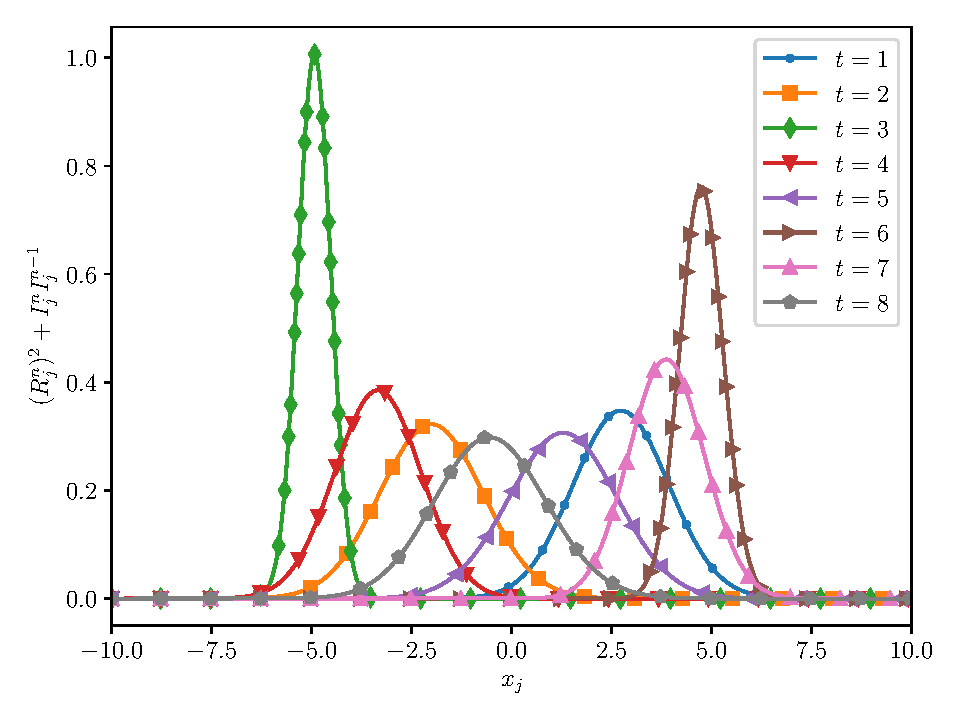
\includegraphics[width=0.8\hsize]{kadai3/main.pdf}
                \caption{Schr\"{o}dinger方程式の解}
                \label{fig:schroedinger}
            \end{figure}

\newpage
\addcontentsline{toc}{section}{参考文献}
\begin{thebibliography}{99}
    \bibitem{text}{
        実験演習ワーキンググループ、``数理工学実験 2022年度版''、京都大学工学部情報学科数理工学コース (2022)
    }
\end{thebibliography}
\end{document}